\subsection{Data and Preprocessing}
The ODDS-Dataset published by \citet{Rayana:2016} is a widley used repository as benchmark datasets.
E.g. \citet{shenkar2022anomaly} use those datasets to identify stregths and weaknesses of a bunch of outlier detection methods, including the above describes InterCont.
The datasets contain 32 datasets wich different amounts of dimensions and instances. 
To take the whole picture of a method, it is beneficial to use a wide range of different datasets, to determine the advantages and disadvantages of a method.
Nevertheless, using upto 32 different datasets is not feasable for my thesis, because it wont be in the scope of this thesis.
Therefore I will analyse the wine dataset in great detail, to use those finding in the result section.
The goal of this section is to anaylse and describe the dataset
Therefor I will first summarize the dataset statistically, including central tendencies, shape, distribution, cardinality and spracity.
Subsequently I will analyse bivariate relationships inside the dataset as well.
Finally I will analyse the geomatric structure of the dataset, including intrinsic dimensionality and manifold structure.


\subsubsection{Introduction}  
\textcolor{red}{Describe what type of data has been collected in the data, How was it collected,What is the ground truth - how are the lables be defined? How are outliers defined in specific context}
The wine dataset was donated from \citet{wine_109} at the 30.06.1991 to the UC Irvibe machine learning Repository.
The authers collected data about chemical components of wine wich came from three different italian wine growers. 
First it was used as a multi classification task dataset, because it had three classes, one for each wine grower.
For outlier detection Shebuti et al tranformed this dataset into an unbalanced binary classification dataset and offered it in the ODDS Repository for general scientific uses. 
129 instances (wines) and 13 variables were left in the remaining dataset.
She combined the wines of wine grower two and three to be the normal class, resulting in 116 wines and wine grower one was defined as the anomaly class, resulting in 10 abnormal wines.
Correspondingly, the outlier ratio is 7,7\% placing it in the \todo{filling the average outlier ratio of ODDS}
Conviently, Shebuto et al excluded all missing data and left only continious instances.
In the following the feature names are not included into the diagrams because of design choices.
To give an clue to wich feature what resembles, here the names of the features: 

\begin{figure}[h]
    \centering
    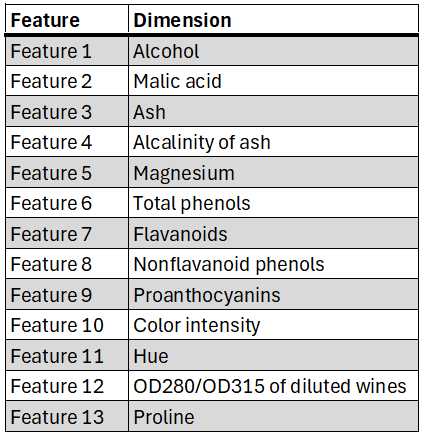
\includegraphics[scale=0.75]{Images/Data/Table_of_Names.pdf}
    \caption{Featurenames}
\end{figure}

\subsubsection{Statistical Summarization}
In this section  I will describe the central tendencies of the dataset, beginning with univariate analysis.
Figure three is depicting boxplots per feature in the dataset.
Depicted is the interquartile distance (IQD), mean, median and the whiskers (1,5*IQD).
The red dotted line is the average and the grey line is the median of the feature.
The average is not robust against outliers, not as the median. 
The difference between the two parameters can be interpreted as skewdness of the distribution. 
If the mean is bigger than the median, the distribution is left skewed.
If the mean is smaller than the median, the distribtion is right skewed.
This is especially pronound for Malic Acid (Feature 2). 
All of the features are left skewed, except of Feature 8 and 12.
But those differences are not as profound as other differences of other features 
Data instances that lay above or under the whiskers are depicted as outliers in a univariate sence.
Some features contain more outliers than other features. 
Only three instances in feature 3 and 4 are outliers because of their small value. 
All the other outliers are defined as outliers because of their large value. 
Per definitionem those outliers could be global outliers, because of their fringe values. 
To further investigate those outliers, I compared the ground truth with the outliers diganosed with the IQR. 
Instances, that are diagnosed outliers and are outliers defined by the ground truth are coloured in red.
Instances that are not coloured are diagnosed outliers but are not in fact outliers.
Those abnormal values can be explained by other dimensions.
By not incorporating the correlations, this methods of outliers detection would be detecting a number of false positives. 



\begin{figure}[h]
    \centering
    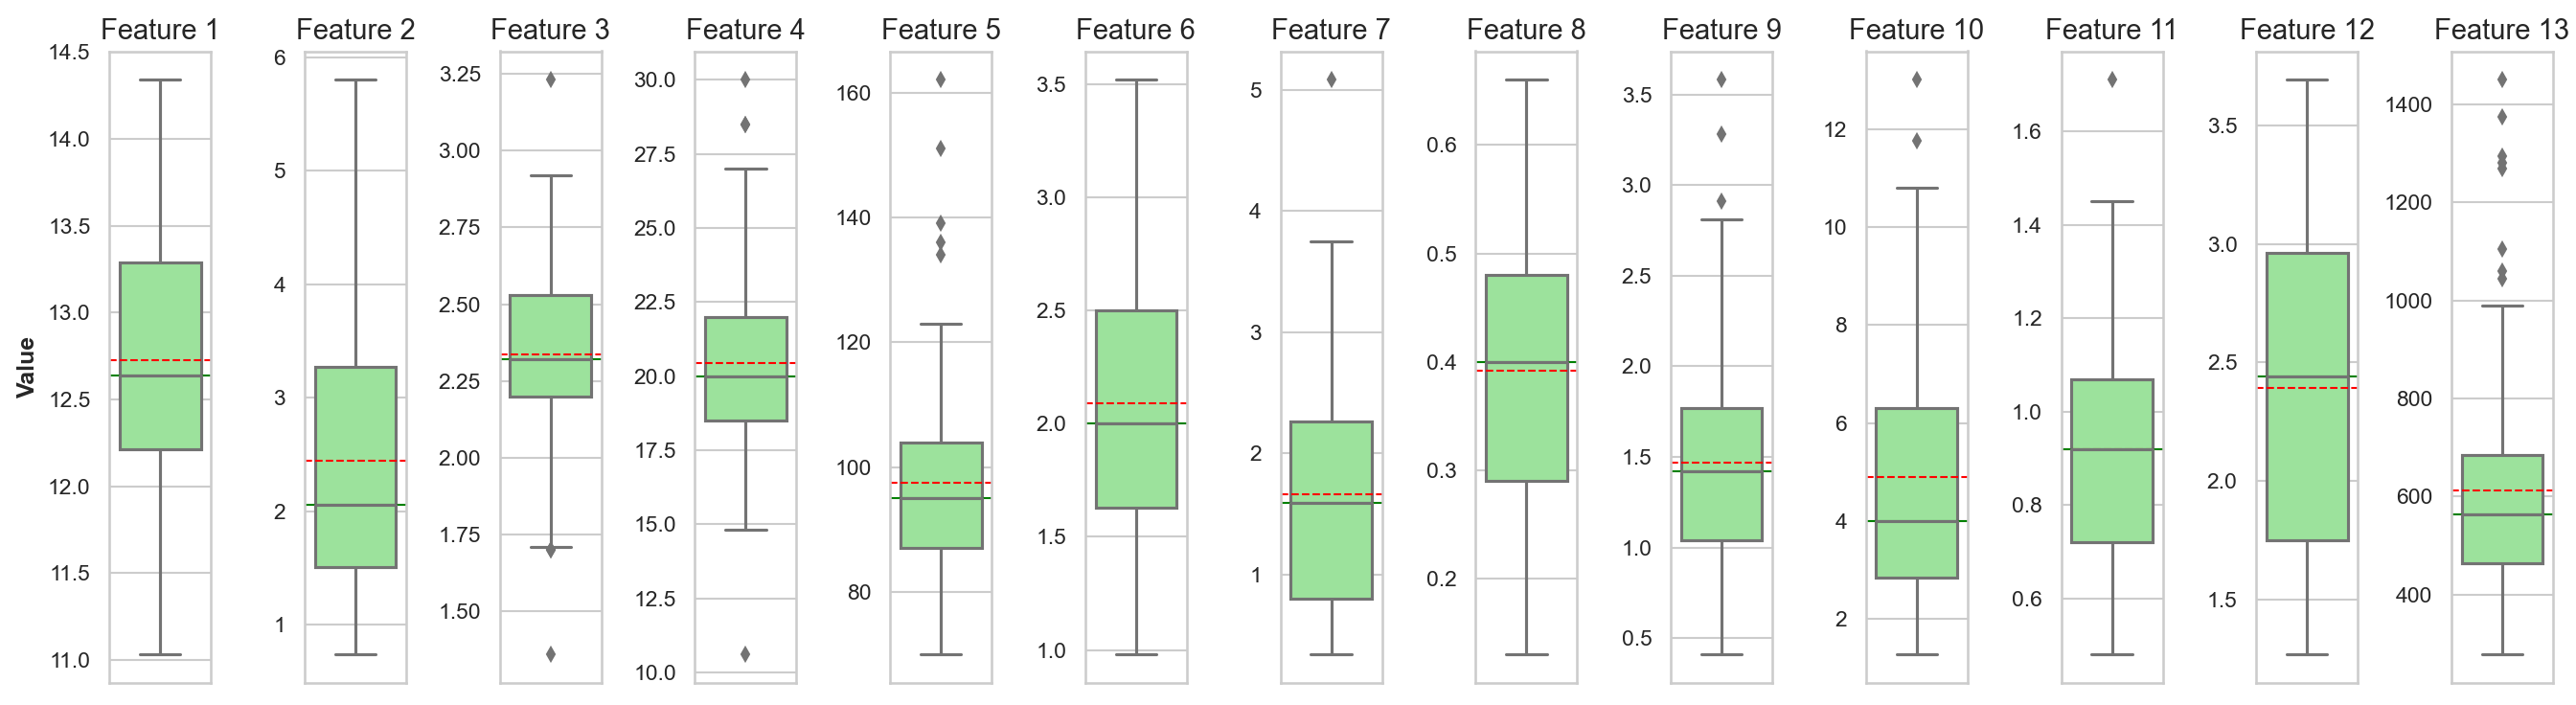
\includegraphics[width=1.0\linewidth]{Images/Data/boxplots.pdf}
    \caption{Boxplots}
\end{figure}

The table depicts the usual boxplots with 1,5*interquartile range, wiskers, mean and median.
In traditional boxplots there are instances shown as outliers, that are more extreme then the 1,5*interquartile range.
I  forgo without them, because this thesis is not about outlier detection in univariante distributions.
The difference in mean and median in all features except feature 1 is neglectable small. 
The boxplot of feature 1 has be more analysed, because the mean and the median differ a lot.
Thats a sign, that feature 1 is skewed to right and distibutions does not follow a normal distribution.


To be statistically sure, I apply the Shapiro-Wilk test for Normality.
The requirements are met.
With 3772 instances the data does not exceed the maximum of 5000 instances and therefore has a reasonable sensitivity.
The underlying distributions have to be in a metric scale level, the data is iid and . 


The Null is H0: 
Nevertheless for every instance the Shapiro-Wilk test for Normality the H0 is rejected. 
None of the 6 instances follows a normal distribution.
For further information the results are placed in the appendix. \todo{display table into appendix}

    Statistical Summarization
        - Central tendencies and dispersion:
            - Mean, variance, standard deviation
        - Shape and distribution:
            - Kurtosis and Skewness
            - Multivariate Normality: Henze-Zirkler test - if data is non normal, statistical methods will fail
            - Modality: Clustering Tendency (Hopkins Statistics) - If data has multiple naturl clusters ,multimodel, global outlier methods will fail 
        - Cardinality and Sparsity:
            - Identify the number of unique values in categorical - High-cardinality categorical variables (like "Zip Code") can create "sparse" 
                regions that look like outliers but are actually just rare valid entries.
            - Sparsity: determine the percentage of missing values across the feature space
            - Visualisation: 
        - Bivariate Analysis
            - Bridge the gap between individual data points and multicolinearity
            - Correlation Matrix: Pearson for linear and Spearman or Kendall for non-linear/rank based relationships
            - Categorical Association: Chi-Square tst or Cramer's V to see specific categories are associated with one other
            - Multicollinearity: VIF
            - Mutual information: identify non-linear dependencies thats standard correlation might miss
       - Visualisation: A table of features, type (numerical/categorical) and cardinality.


    Geomatric structure
        high dimensional data rearly is uniformly
        - Intrinstic dimensionality (ID): 
            - Definition: ID is the minimum number of variables (or dimensions) required to represent the essential information within datatset and without significant loss.
                is the variance just drivenby a small number of data
            - Problem: Curse of Dimensionality. The volume of the space increases so fast that the data becomes sparse
                If your dataset has 50 variables but 95\% of the variance is captured by 3 variables, the "curse of dimensionality" is low, and simple methods (like Mahalanobis Distance) might beat complex ones (like Isolation Forest).
            - Visualization: Heatmap, Use a method like the Scree Plot from PCA
        - Manifold structure: Is the data on a curved surface or is it clustered
            - Definition: manifold structure refers to the hypothesis that high dimensional data actually lives on a mich simpler, lower-dimensional surface embedded within that high-dimensional space
            - Problem: Traditional distances fail on manifold. If two points are on the opposide side of a fold, they might look close in 3D space, but they are actually very far apart along the surface of the paper.
            - Impact: A data point miht look like an outlier in 3D becaus its away from the center, but is perfectly normal when you follow the flow of the manifold. 
                or the opposite. A point could be inside thedata cloud but odd the manifold surface - making a hidden outlier
            - Analyze: Estimate Intrinsic Dimensionality using Maximum Likelihood Estimation of intrinsic dimension
            - Visualization: t-SNE plot or UMAP, those are specifically designed to unfold the manifold so you can see 2D structure 
            - Result: if the manifold are varying in density, a global method (T-Score) will fail, Manifold aware methods are more suitable (LOF) 
            
            
    Preprocessing and transformation
        - Multicollinearity: PCA
        - Missing values: how to handle
        - High cardinality: Noralization

\subsubsection{The Problem of synthetic data}
\textcolor{red}{ Take on here }
    Revisiting Time Series Outlier Detection: Definitions and Benchmarks (Lai et al., 2021)
        Most synthetic data is generated by adding Gaussian noise or simple "spikes" to a clean signal
        he paper found that many deep learning models achieve near-perfect scores on synthetic data but perform worse than 30-year-old classical methods (like Isolation Forest) on real data. 
        This is because synthetic outliers are often too easy to distinguish from the normal distribution, leading to "inflated" performance metrics
    Synthetic Data, Synthetic Trust: Navigating Data Challenges in the Digital Revolution
        Researchers often develop an unwarranted confidence in models trained on artificial data.
        Synthetic generators (like GANs or VAEs) often fail to capture rare, complex correlations between variables (Intersectional Fidelity). 
        If the generator hasn't seen a specific type of rare "multi-variable" outlier, it won't produce it, and your model will never learn to detect it
    An Empirical Analysis of Synthetic-Data-based Anomaly Detection (Llugiqi  Mayer, 2022)
        In synthetic datasets, the "normal" data is often too "clean."
        Real-world data is naturally "messy" (sensor jitter, network lag). In synthetic benchmarks, the boundary between "Normal" and "Outlier" is mathematically sharp. 
        In the real world, that boundary is fuzzy.
        A model trained/benchmarked on synthetic data might treat any slight real-world noise as a "High-Confidence Outlier," leading to a flood of false positives in production.
  
